\chapter{Results}
This results chapter is meant as a mechanism to present all of the data that was collected on the performance of different demodulators. All of the demodulators that were tested in the course of this research will be shown, whether it be dedicated hardware or software. The first results that will be shown are those of the dedicated hardware, being TNCs and Argent Data's OpenTrackers. Following the hardware will be the software implementations. Following these two categories will be some general comparisons between them.

\section{Dedicated Hardware Results}
In the scope of this research a total of 12 pieces of hardware were tested. They include Argent Data's OpenTracker 2, OpenTracker 3, OpenTracker USB, OpenTracker 3 Micro, Kantronics Kam, two Kantronics Kam Plus, two AEA PK-88, a PK-232, a PK-232MBX, and an MFJ-1278. Hardware models for which more than one was tested will be differentiated by a number in parentheses following the model number. Please note that on the figures OpenTracker will be abbreviated OT.

The first two tests consisting of clean packets - 40 generated from the OpenTracker and 200 using Toledo's suite - was relatively uninteresting. Essentially every piece of hardware decoded all 40 and all 200 packets. The only anomalies to this were that the OpenTracker USB was only able to decode 39 and 193 out of the 40 and 200 packet files respectively. Additionally the OpenTracker 3 Micro missed one packet in the 200 packet file to only decode 199. Since there is no real way to debug and see the cause of decoding relatively fewer or more packets just the data for these hardware items is presented as it was measured to allow for comparison to the software. This will continue to be the case for the remainder of this hardware section.

Following the two easy files the next file is same content as the file with 40 packets in it, with the only difference being that noise was progressively added. In Figure \ref{allHardwareOT3Noise}, the two PK-88s stand out for being able to decode 25 of the 40 packets in this file.

 \begin{figure}
  \centering
	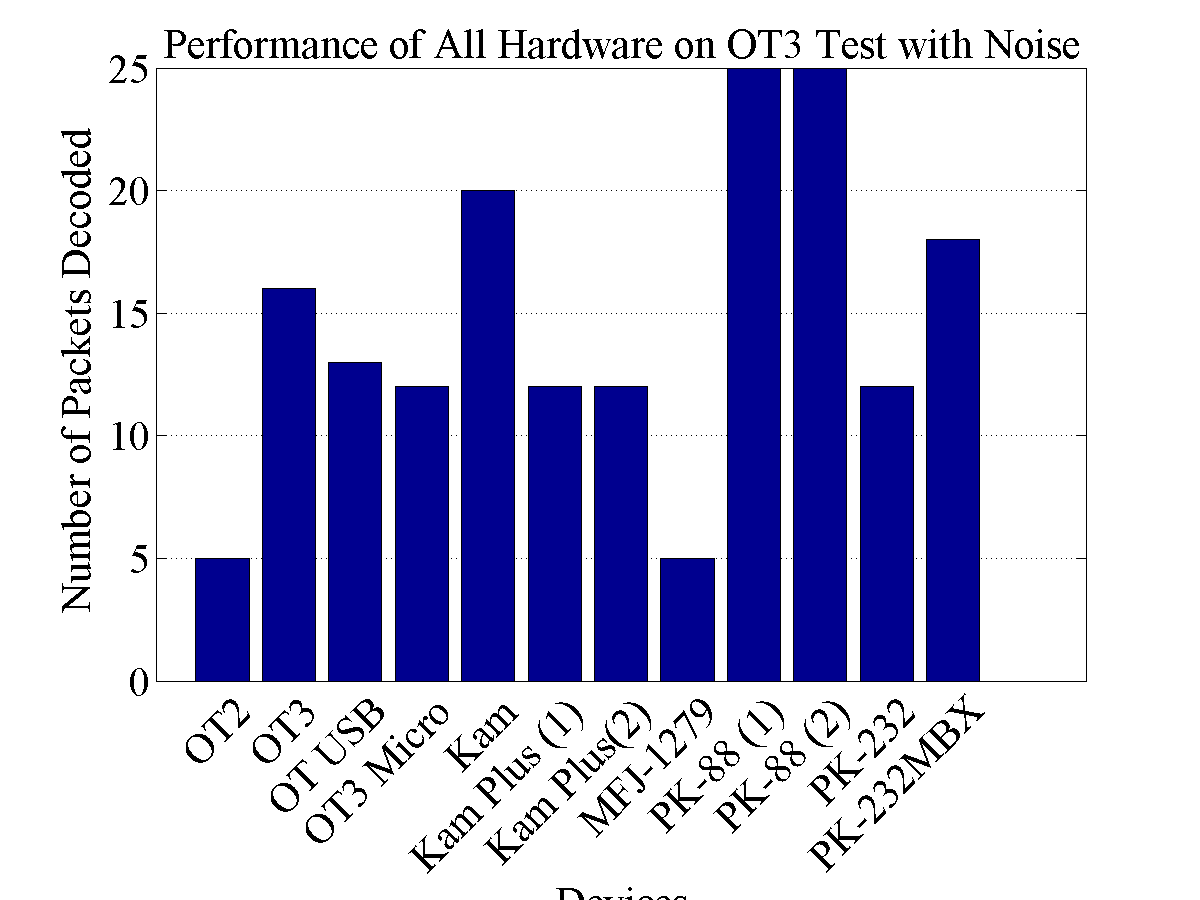
\includegraphics[width=0.75\linewidth]{images/PerformanceofAllHardwareonOT3TestwithNoise.png} 
	\caption{Number of packets successfully decoded for all tested hardware on the OpenTracker 3 test file with noise.}
   \label{allHardwareOT3Noise}
\end{figure}

The next two files are the ones that were used most extensively in the testing for comparison and tuning. Primarily the first, which is just a recording of traffic off the air. They are Track 1 and 2 from the APRS CD mentioned in the Demodulator Benchmarking Chapter. The results from Track 1 are in Figure \ref{allHardwareTrack1} and Track 2 in Figure \ref{allHardwareTrack2}. The top three performances of the hardware on Track 1 were the PK-88 (2) with 1007 packets decoded, the Kam with 988 Packets, and the Kam Plus (2) with 985 Packets. For Track 2 the top hardware was the Kam Plus (2) with 998, the Kam Plus (1) with 967, and the Kam with 938.

 \begin{figure}
  \centering
	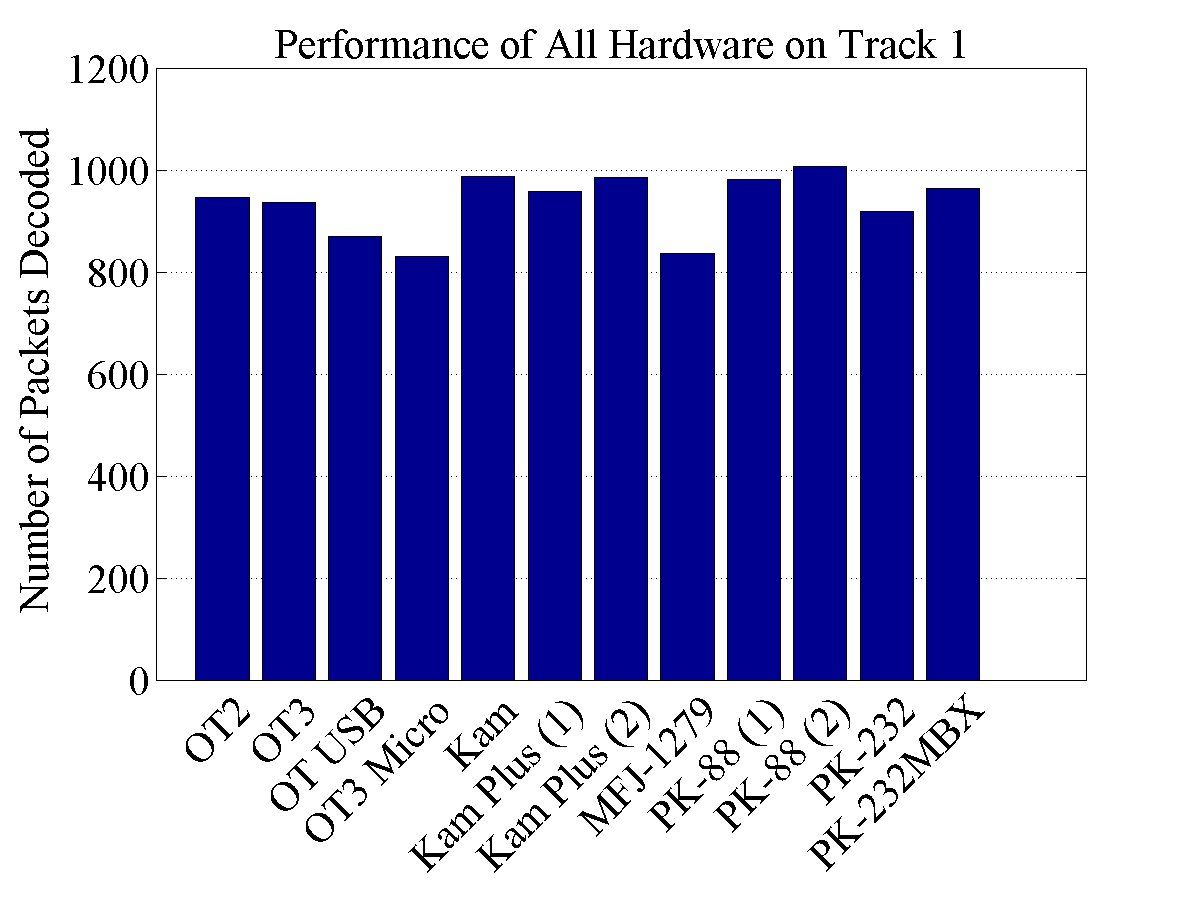
\includegraphics[width=0.75\linewidth]{images/PerformanceofAllHardwareonTrack1.png} 
	\caption{Number of packets successfully decoded for all tested hardware on the Track 1 test file.}
   \label{allHardwareTrack1}
\end{figure}

 \begin{figure}
  \centering
	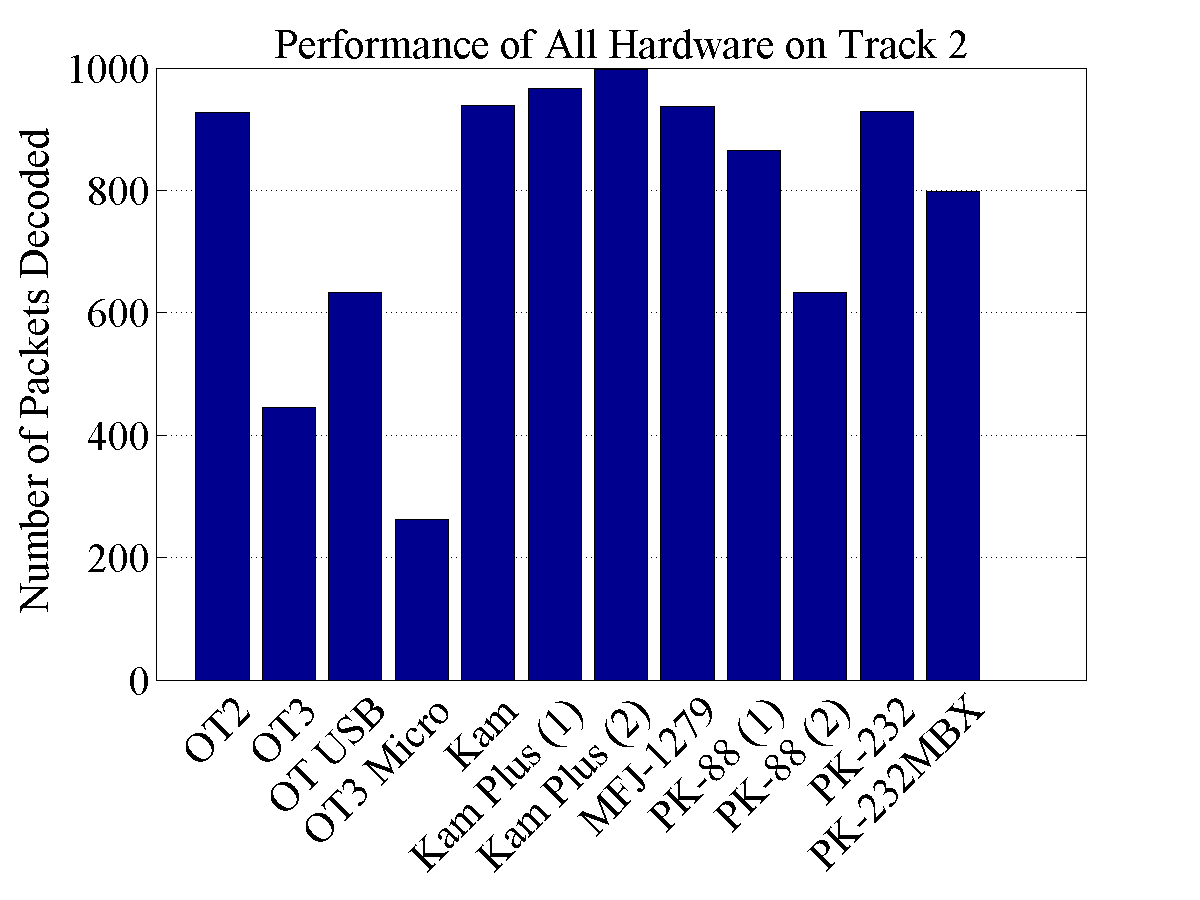
\includegraphics[width=0.75\linewidth]{images/PerformanceofAllHardwareonTrack2.png} 
	\caption{Number of packets successfully decoded for all tested hardware on the Track 2 test file.}
   \label{allHardwareTrack2}
\end{figure}

Using these results the best numbers for the hardware were 40 packets decoded from the Open Track 3 test, 200 from the javAX25 generated file, 25 from the Open Tracer 3 test with added noise, 1007 from Track 1 of the LA test suite, and 998 from Track 2. These best results can be used as a comparison for the software.

\section{Software Results}
In this section the number of packets that each of the demodulators in the javAX25 package was able to decode will be presented, highlighting those that were newly implemented in the course of this research. This will include the correlation approach that was already implemented before the start of this research as well as all of the new algorithms that were outlined in the previous chapter on Implementation. However, before getting the results from javAX25 there is one more data set to be introduced which is the results from another software based demodulation from AGW Packet Engine. Using this software 40 packets were decoded from the OpenTracker 3 test, 200 from the javAX25 generated file, 21 from the OpenTracker 3 test with added noise, 967 from Track 1 of the LA test suite, and 497 from Track 2. The results from javAX25 end up being on par with these results as well as those of the hardware.

With a total of 13 algorithms implemented, some did well and others not at all, so as in the section on hardware results, all of the data will be presented followed by a focus on those that performed the best. In the new javAX25 software implementation the filtering was moved from its original location of being on a per demodulator level basis to a central location that allowed each of the algorithms to utilize it. Some of the algorithms ended up relying on it after tuning and others could remain independent. As such, in order to present all of the data each algorithm will not only have a result for each of the 5 test files, but also for each of the three filters used on the data. The three filters used are no filter, a 900-2500Hz bandpass filter, and the same bandpass with a 6dB attenuation of 1200Hz tones to combat the signals that were not emphasized when transmitted but were deemphasized when received. For instance, for the Zero Crossing demodulator there will be three values for the OpenTracker 3 Test file, one at each filtering, and so on for the remaining 4 test files.

In terms of the data, correlation data will be on the far left of all the plots which was the current algorithm that it was the goal to beat. The performance of no filter on the OpenTracker 3 Test can be seen in Figure \ref{OT3FiltNo}, Figure \ref{OT3Filt0} shows data with the bandpass filter, and the emphasizing filter results in Figure \ref{OT3Filt6}. It can be observed that zero crossing did not favor the filters, others were resilient, and preclocking thrived. The Generated 200 Test file is the only file that the peak demodulator performed comperably to the other techniques on. The unfiltered data from this test is in Figure \ref{Gen200FiltNo}, the bandpass data in Figure \ref{Gen200Filt0}, and the results of emphasizing the signal in Figure \ref{Gen200Filt6}. Although the generated 200 packet file and the OpenTracker test file had similar results, the results for the generated 200 were better. This can be attributed to the fact that this file has only ever existed in the digital realm, it was made and consumed there, as opposed to existing in the physical world and then recording it.

\begin{figure}
  \centering
	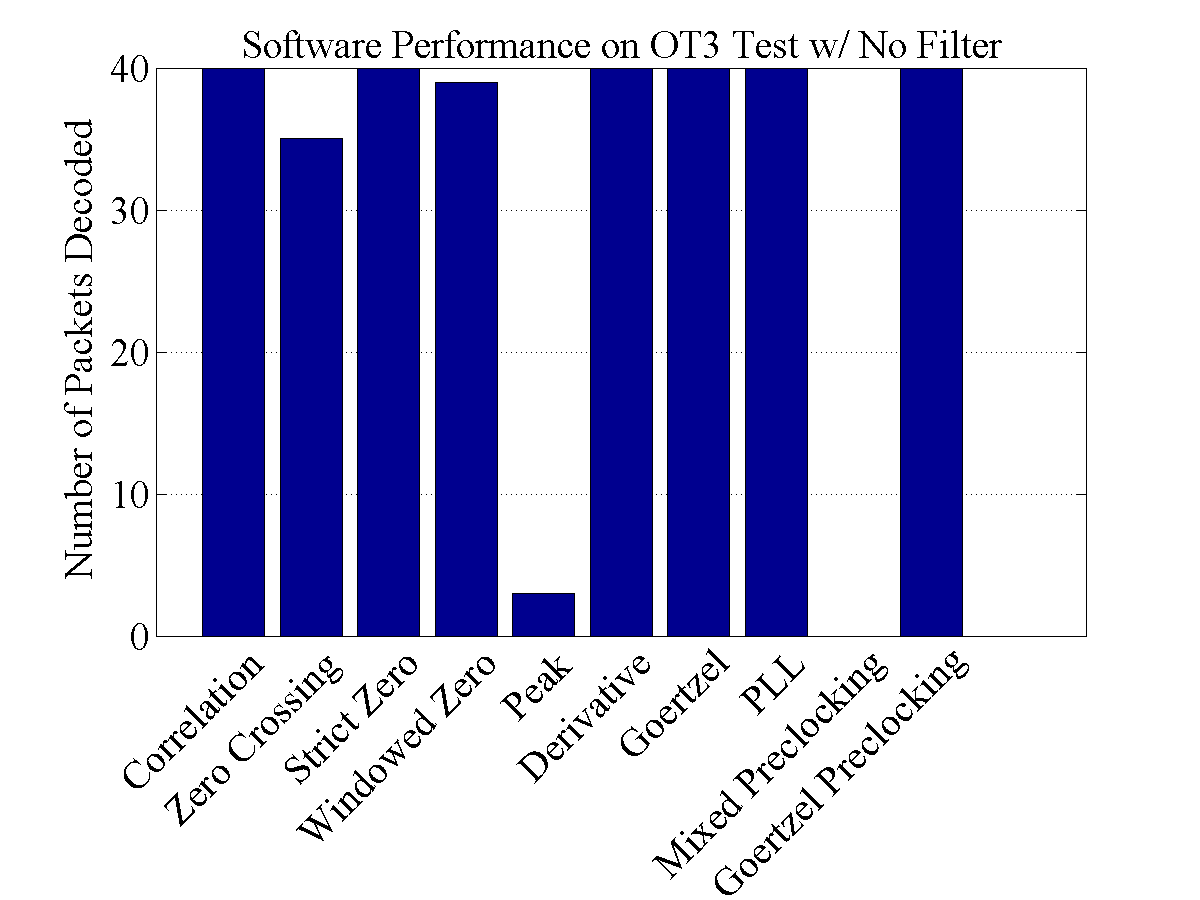
\includegraphics[width=0.75\linewidth]{images/SoftwarePerformanceonOT3TestwNoFilter.png} 
	\caption{Performance of software on the raw signal from OpenTracker 3 Test.}
   \label{OT3FiltNo}
\end{figure}
\begin{figure}
  \centering
	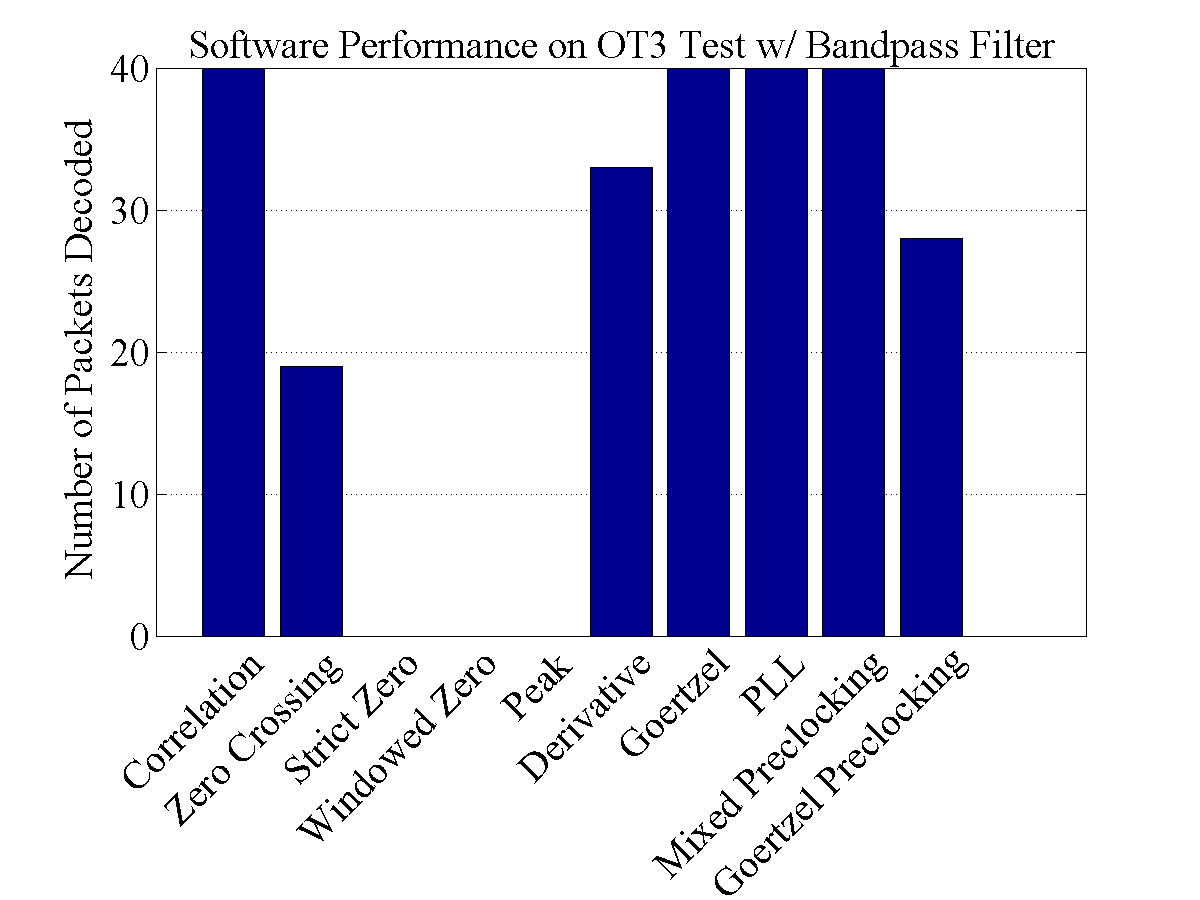
\includegraphics[width=0.75\linewidth]{images/SoftwarePerformanceonOT3TestwBandpassFilter.png} 
	\caption{Performance of software on OpenTracker 3 Test with a bandpass filter.}
   \label{OT3Filt0}
\end{figure}
\begin{figure}
  \centering
	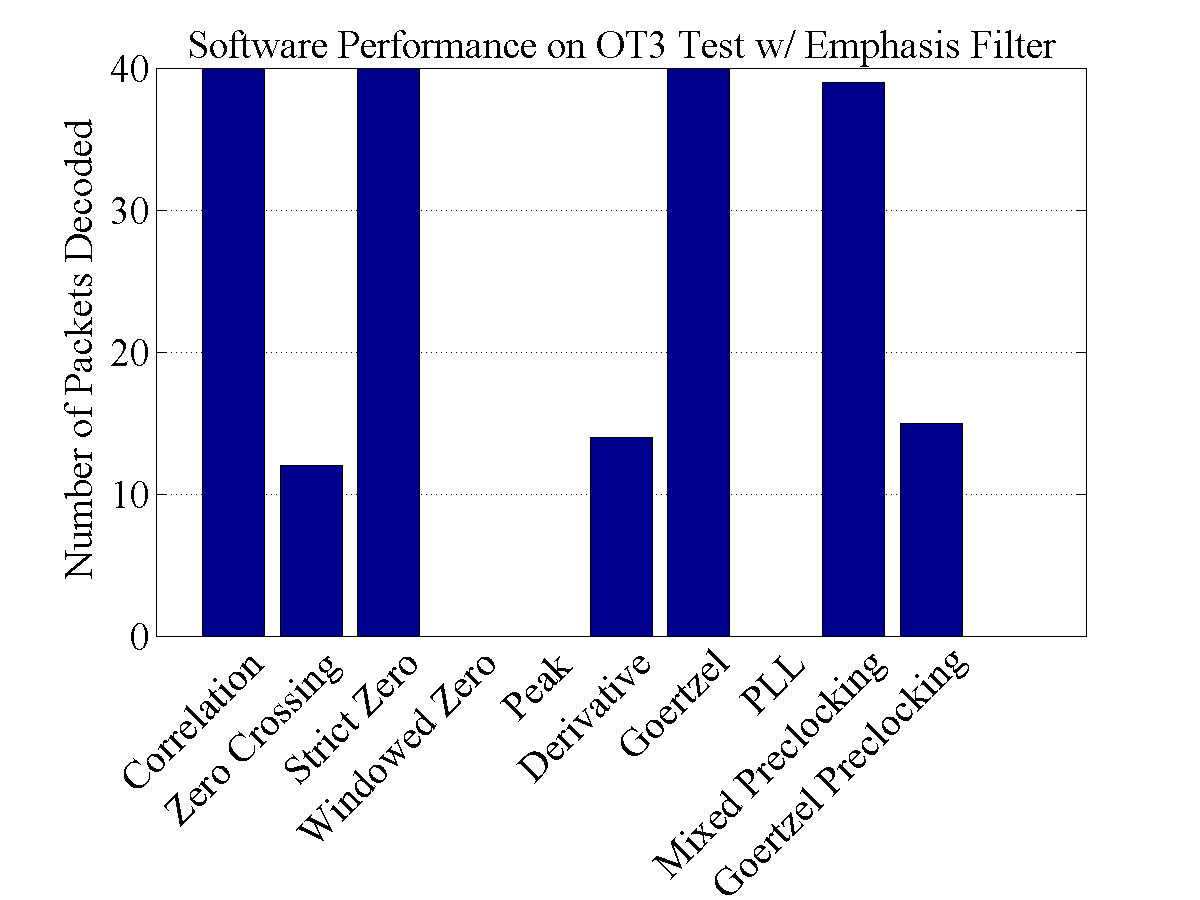
\includegraphics[width=0.75\linewidth]{images/SoftwarePerformanceonOT3TestwEmphasisFilter.png} 
	\caption{Performance of software on OpenTracker 3 Test with an emphasis filter.}
   \label{OT3Filt6}
\end{figure}
\begin{figure}
  \centering
	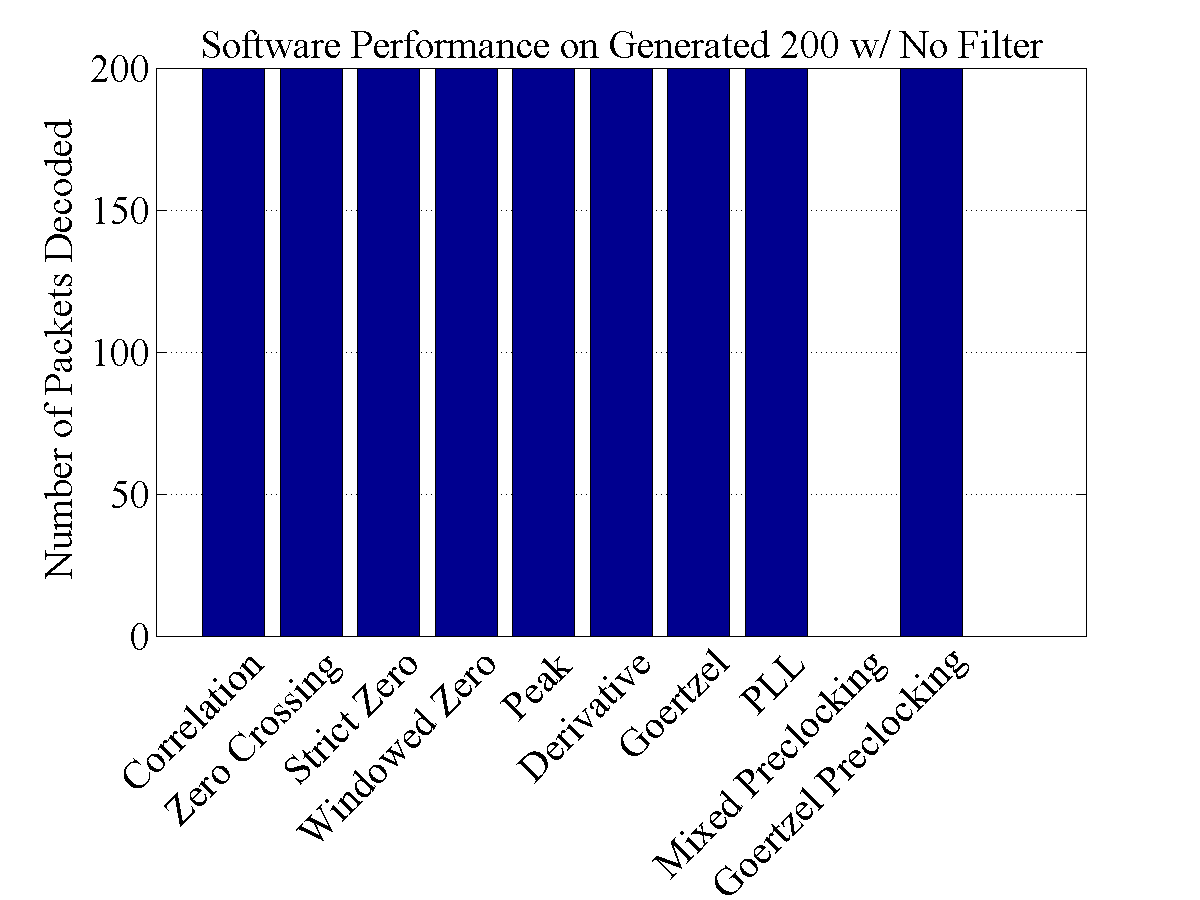
\includegraphics[width=0.75\linewidth]{images/SoftwarePerformanceonGenerated200wNoFilter.png} 
	\caption{Performance of Software on the raw signal from Generated 200.}
   \label{Gen200FiltNo}
\end{figure}
\begin{figure}
  \centering
	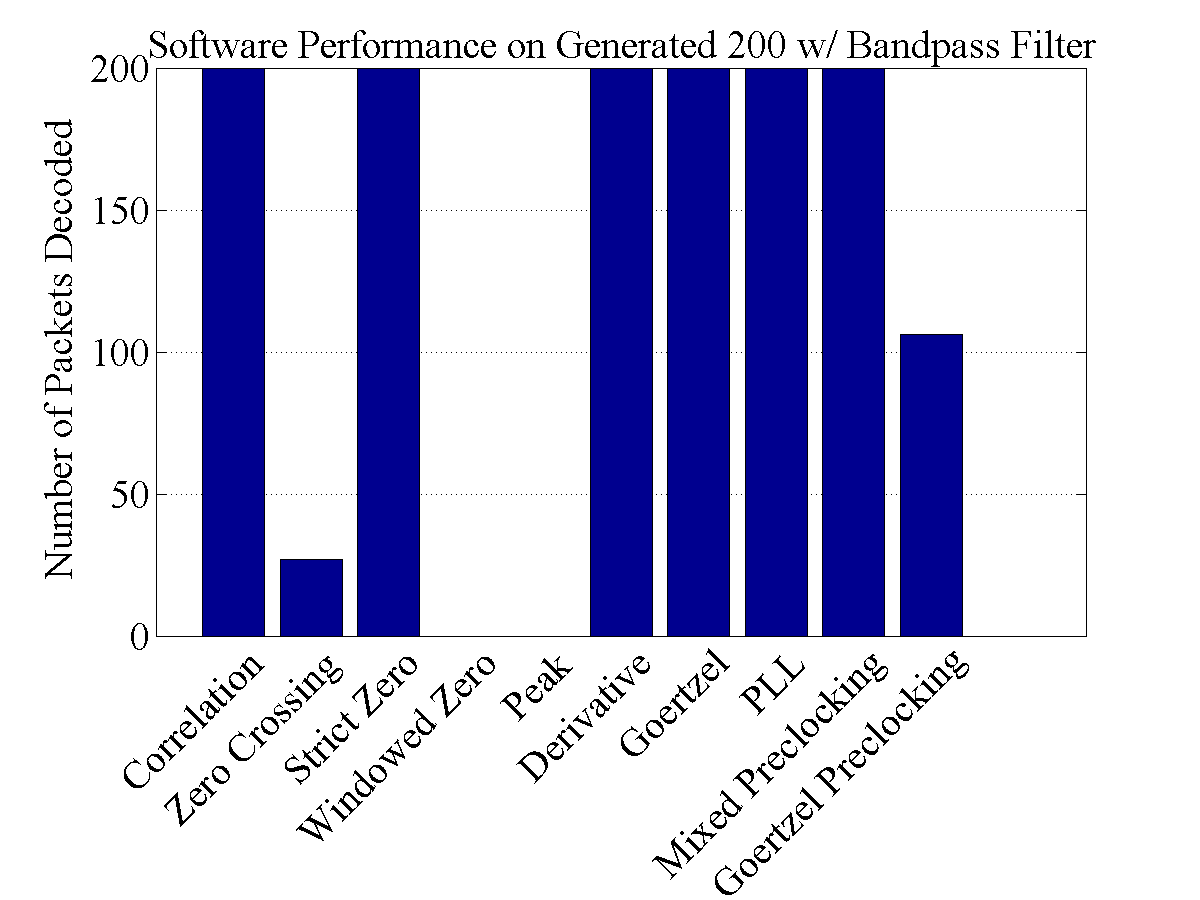
\includegraphics[width=0.75\linewidth]{images/SoftwarePerformanceonGenerated200wBandpassFilter.png} 
	\caption{Performance of software on Generated 200 with a bandpass filter.}
   \label{Gen200Filt0}
\end{figure}
\begin{figure}
  \centering
	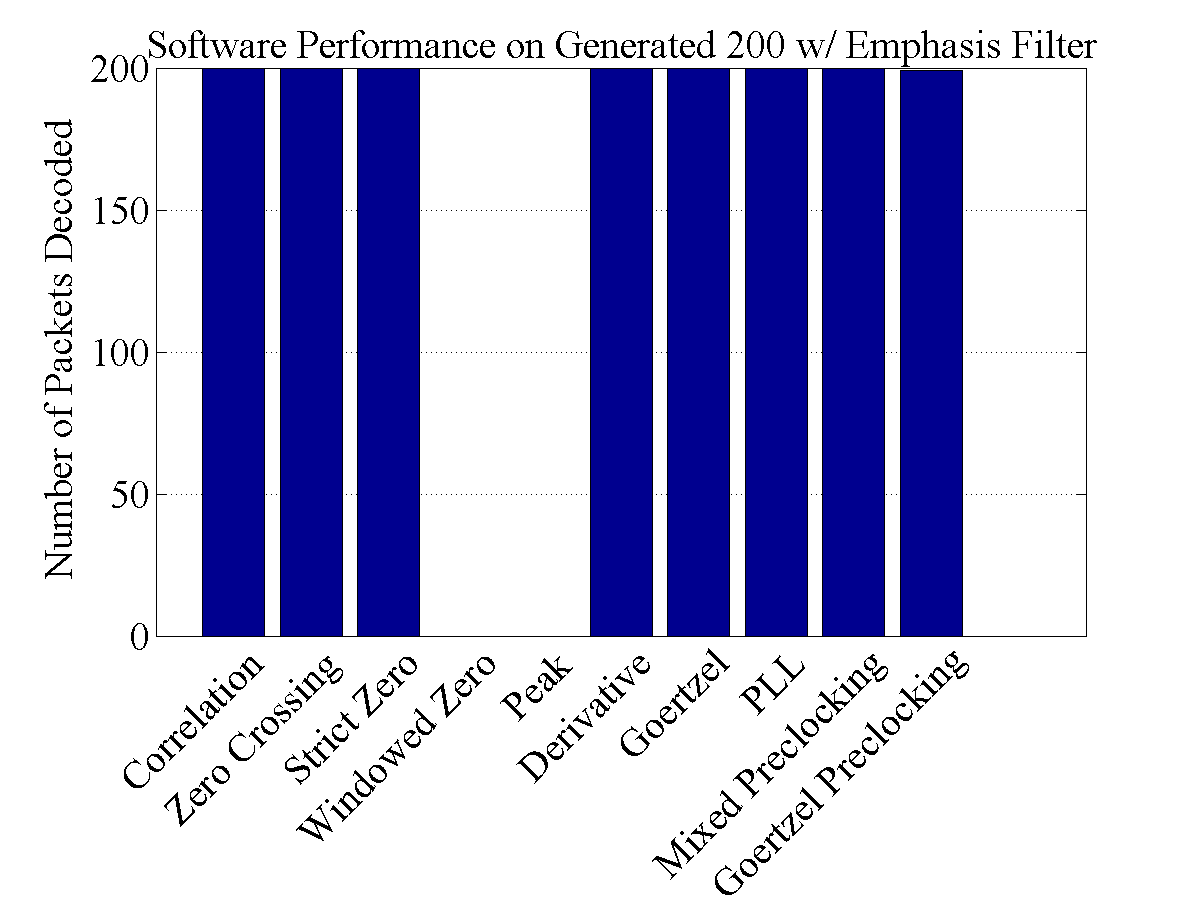
\includegraphics[width=0.75\linewidth]{images/SoftwarePerformanceonGenerated200wEmphasisFilter.png} 
	\caption{Performance of Software on Generated 200 with an emphasis filter.}
   \label{Gen200Filt6}
\end{figure}

Again, moving on from the "easy" files the performance of the software demodulators on the OpenTracker 3 Test with the noise added can be seen. Figure \ref{OTNoiseFiltNo} shows the data for the unfiltered file, Figure \ref{OTNoiseFilt0} shows bandpass filter data, and Figure \ref{OTNoiseFilt6} shows data from the emphasis filter. Two algorithms really start to shine as being comparable, and in some cases better, than the correlation demodulator. Those are the Goertzel Filter Demodulator and the PLL Demodulator. Although this is not data that was actually transmitted or received, these two start so who promise. Even the Strict Zero crossing can be seen doing well once the audio file is emphasized, but it doesn't stand up to the competition in the next two test files.

\begin{figure}
  \centering
	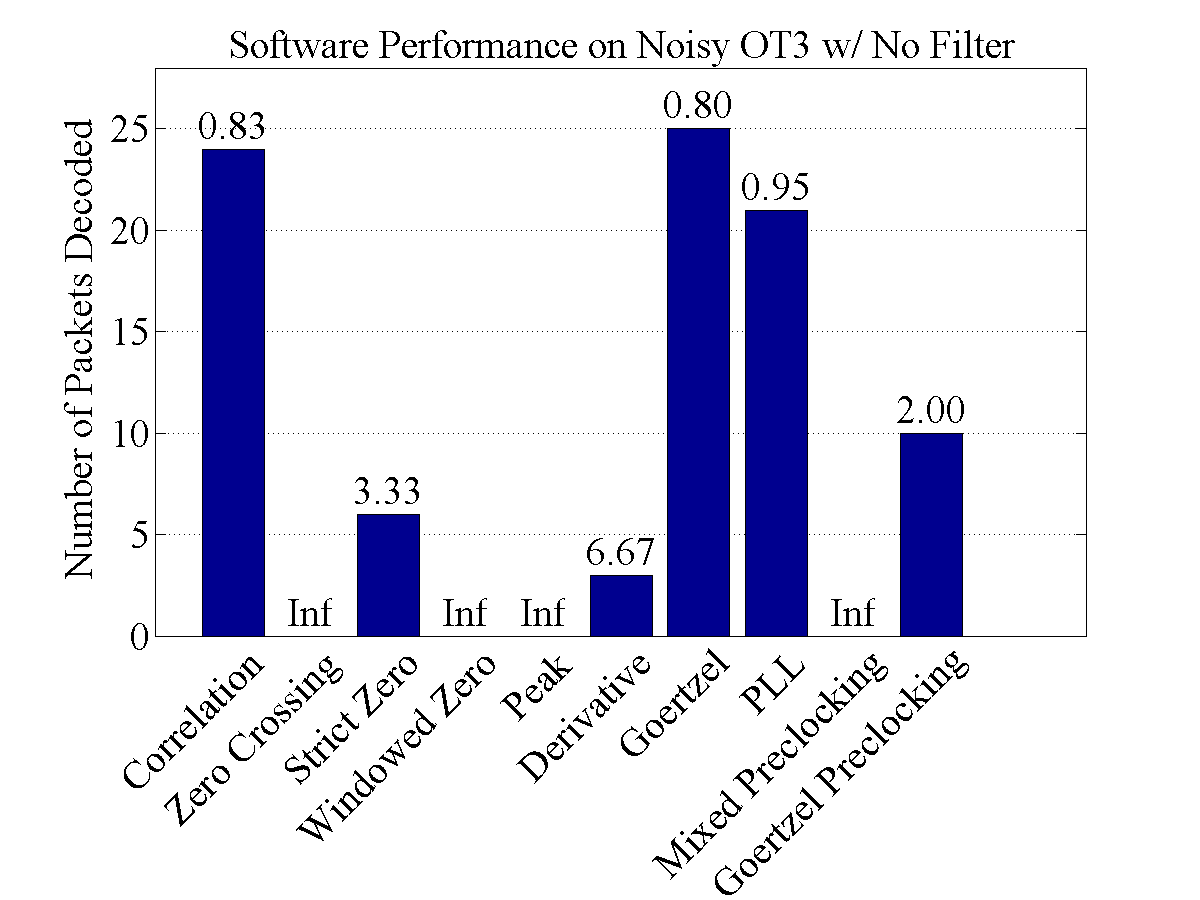
\includegraphics[width=0.75\linewidth]{images/SoftwarePerformanceonNoisyOT3wNoFilter.png} 
	\caption{Performance of software on the raw signal from OpenTracker Test with noise added.}
   \label{OTNoiseFiltNo}
\end{figure}
\begin{figure}
  \centering
	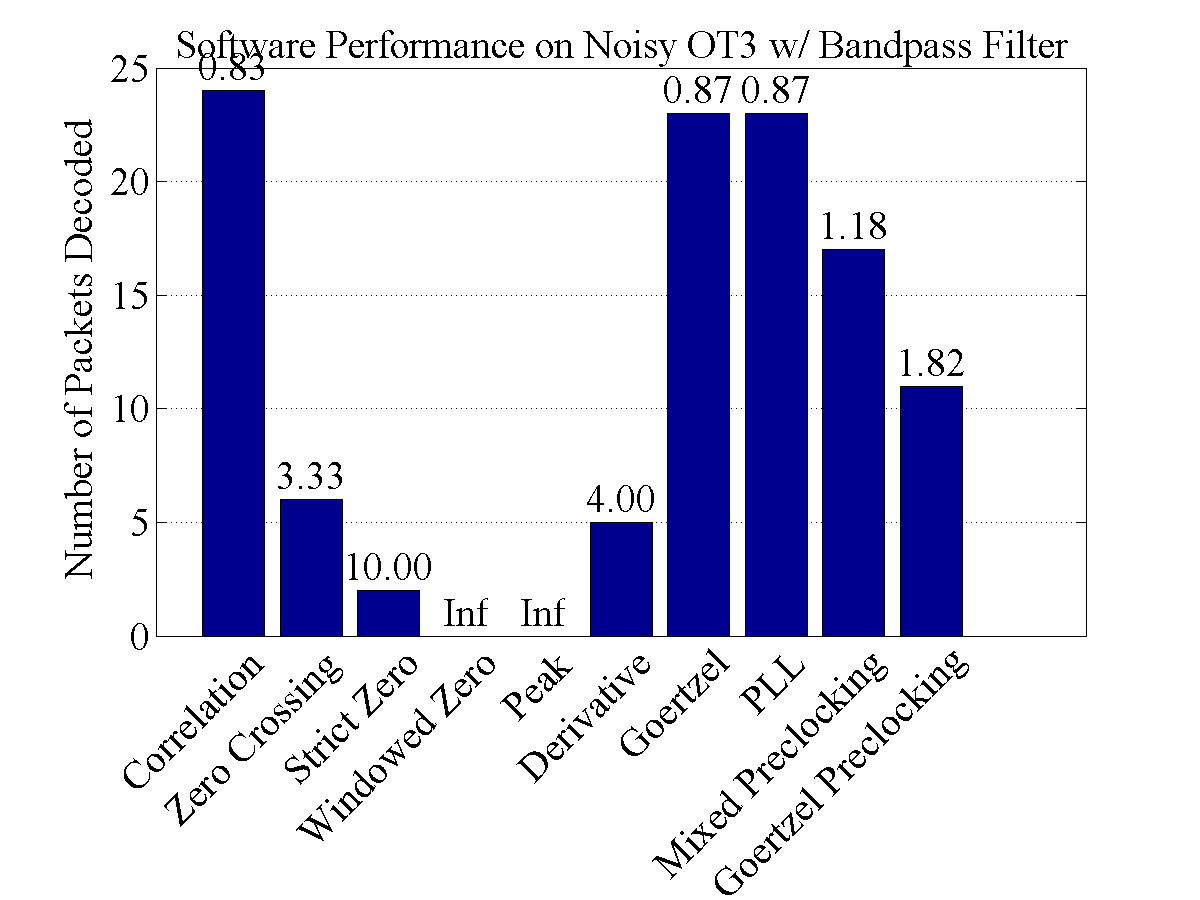
\includegraphics[width=0.75\linewidth]{images/SoftwarePerformanceonNoisyOT3wBandpassFilter.png} 
	\caption{Performance of software on OpenTracker Test with noise added with a bandpass filter.}
   \label{OTNoiseFilt0}
\end{figure}
\begin{figure}
  \centering
	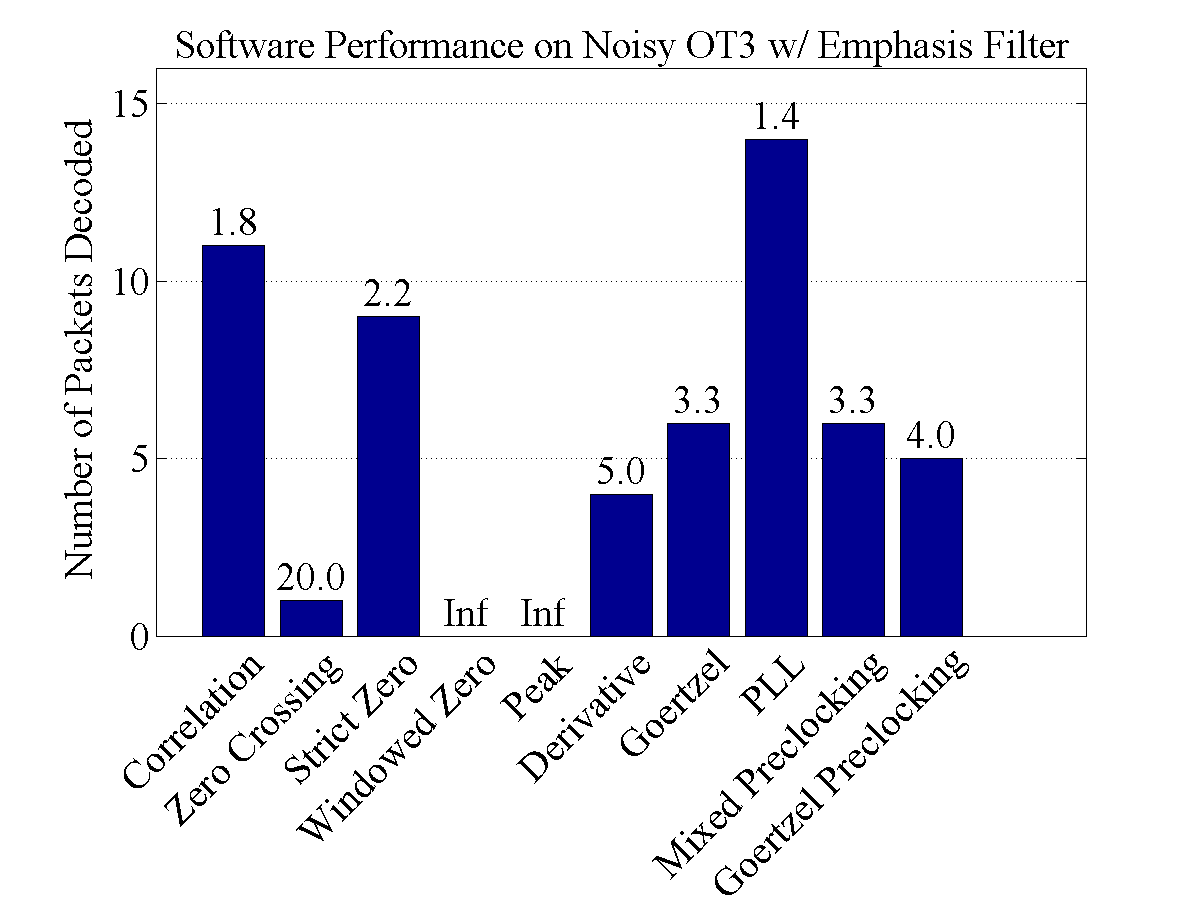
\includegraphics[width=0.75\linewidth]{images/SoftwarePerformanceonNoisyOT3wEmphasisFilter.png} 
	\caption{Performance of Software on OpenTracker Test with noise added with an emphasis filter.}
   \label{OTNoiseFilt6}
\end{figure}

As mentioned earlier, these next two test files were those that were thought the be most important to succeed at. As such, Track 1 was used to tune the algorithms since this would represent the closest real-world simulation possible. The Track 2 results are also presented for comparison. However in Track 2, in addition to being deemphasized the process of this filtering also reduced the magnitude of the signal in the audio file. As such, this file shows two things: One, the ability to pick up lower level signal and second, the algorithms tolerance to signals that were not emphasized when transmitted, but were deemphasized when received. The results of no filtering, bandpass filtering, and emphasis filtering can be seen in their respective Figure \ref{T1FiltNo}, \ref{T1Filt0}, and \ref{T1Filt6} for Track 1. The data from demodulating Track 2 can be seen in Figure \ref{T2FiltNo}, \ref{T2Filt0}, and \ref{T2Filt6}. As was caught during the OpenTracker 3 Test with noise it can be noticed that the Goertzel and PLL algorithms are still doing well on Track 1, and also the Mixed preclocking is doing fairly well. With the filter that is applied on Track 1 to create Track 2 it is basically the opposite effect of Toledo's emphasis filter and hence they cancel each other out. This can be seen by looking at the performance of the Goertzel Demodulator which does poorly with both other filterings on Track 2. However, its ability to detect low level signals and this reversal of the emphasis filtering applied makes it end of having comperable results to the just band pass filter on Track 1 - 956 versus 965. 

\begin{figure}
  \centering
	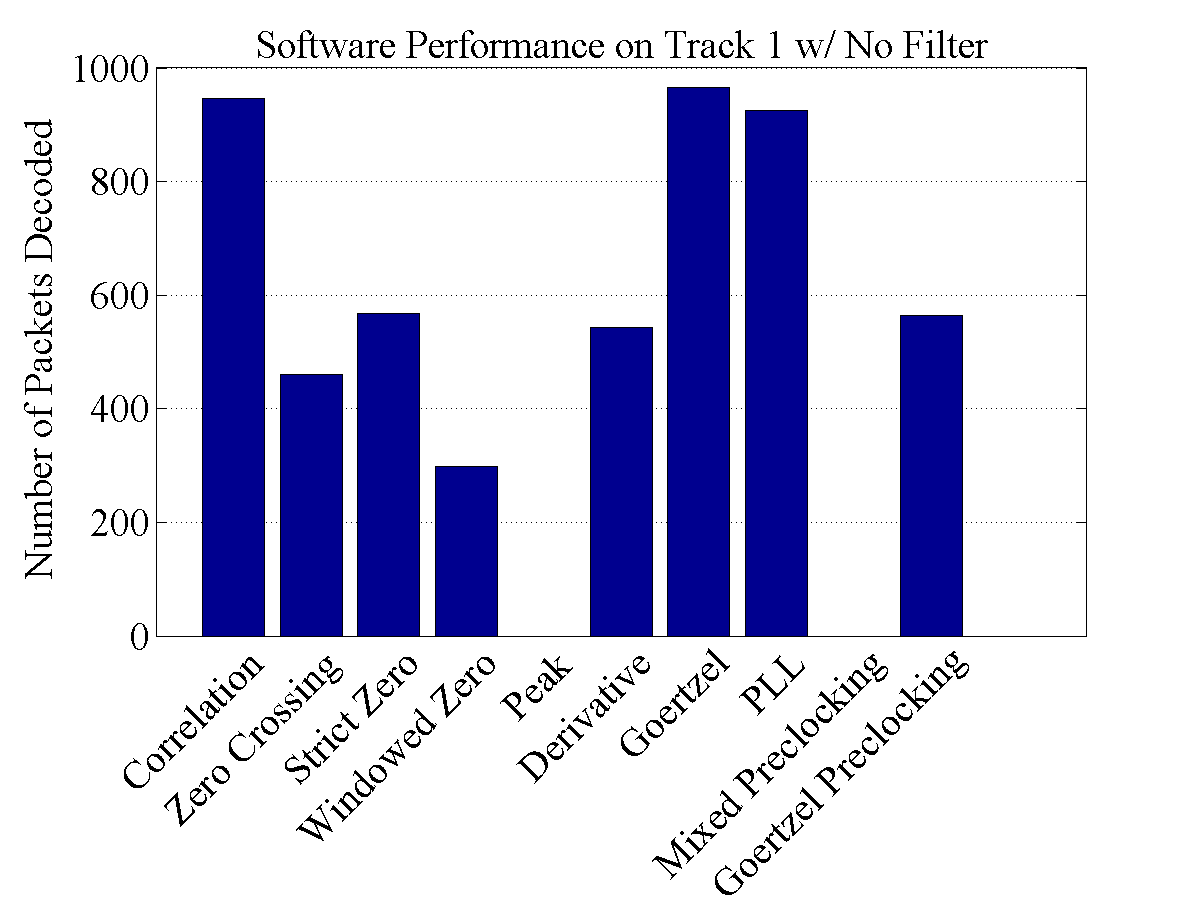
\includegraphics[width=0.75\linewidth]{images/SoftwarePerformanceonTrack1wNoFilter.png} 
	\caption{Performance of software on the raw signal from Track 1.}
   \label{T1FiltNo}
\end{figure}
\begin{figure}
  \centering
	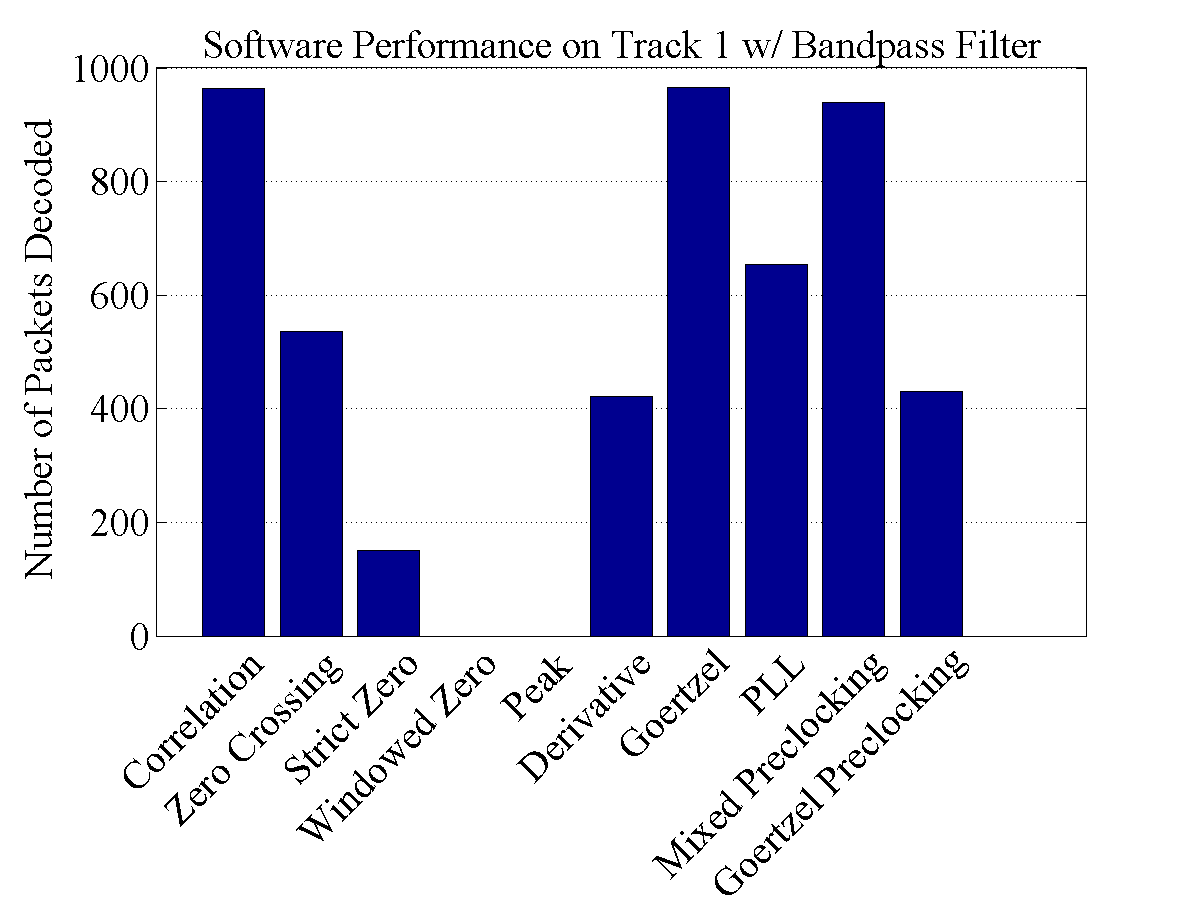
\includegraphics[width=0.75\linewidth]{images/SoftwarePerformanceonTrack1wBandpassFilter.png} 
	\caption{Performance of software on Track 1 with a bandpass filter.}
   \label{T1Filt0}
\end{figure}
\begin{figure}
  \centering
	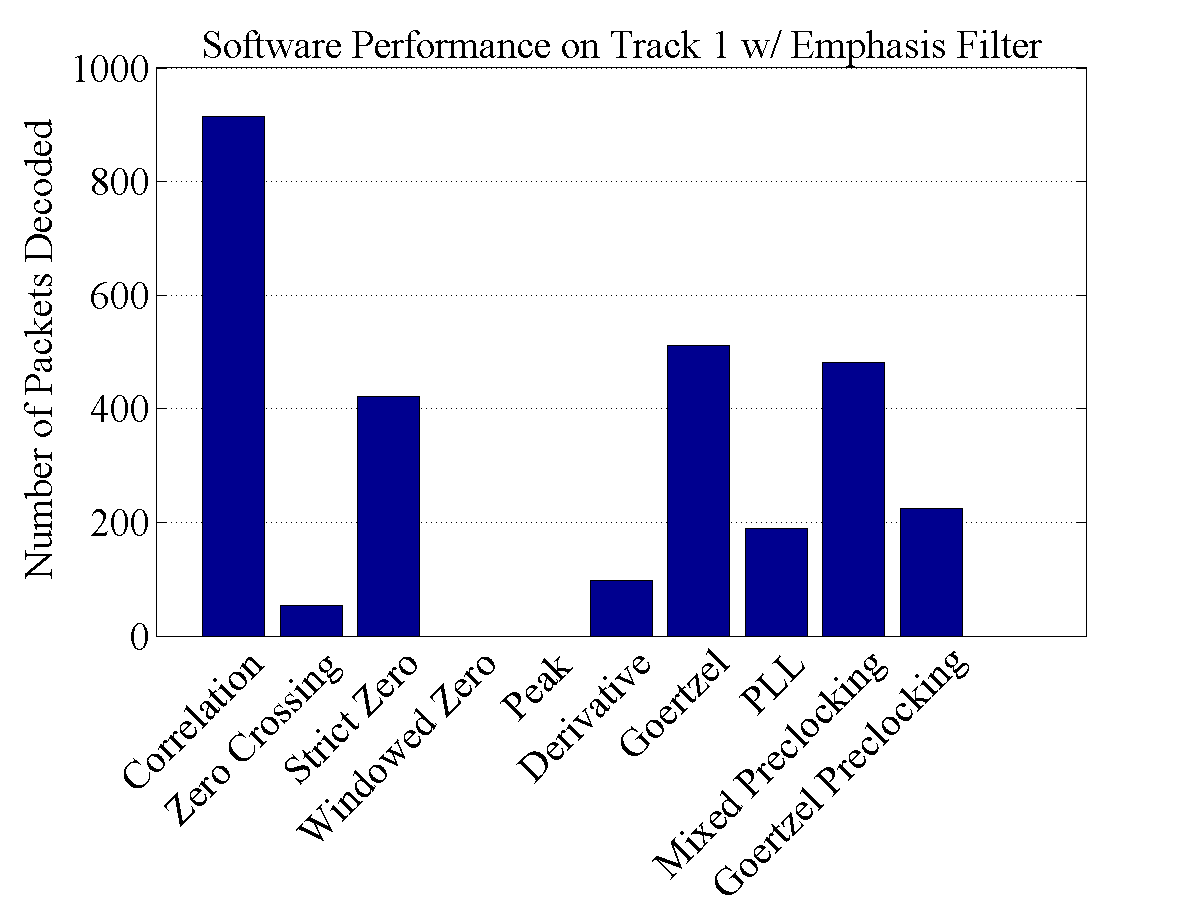
\includegraphics[width=0.75\linewidth]{images/SoftwarePerformanceonTrack1wEmphasisFilter.png} 
	\caption{Performance of software on Track 1 with an emphasis filter.}
   \label{T1Filt6}
\end{figure}
\begin{figure}
  \centering
	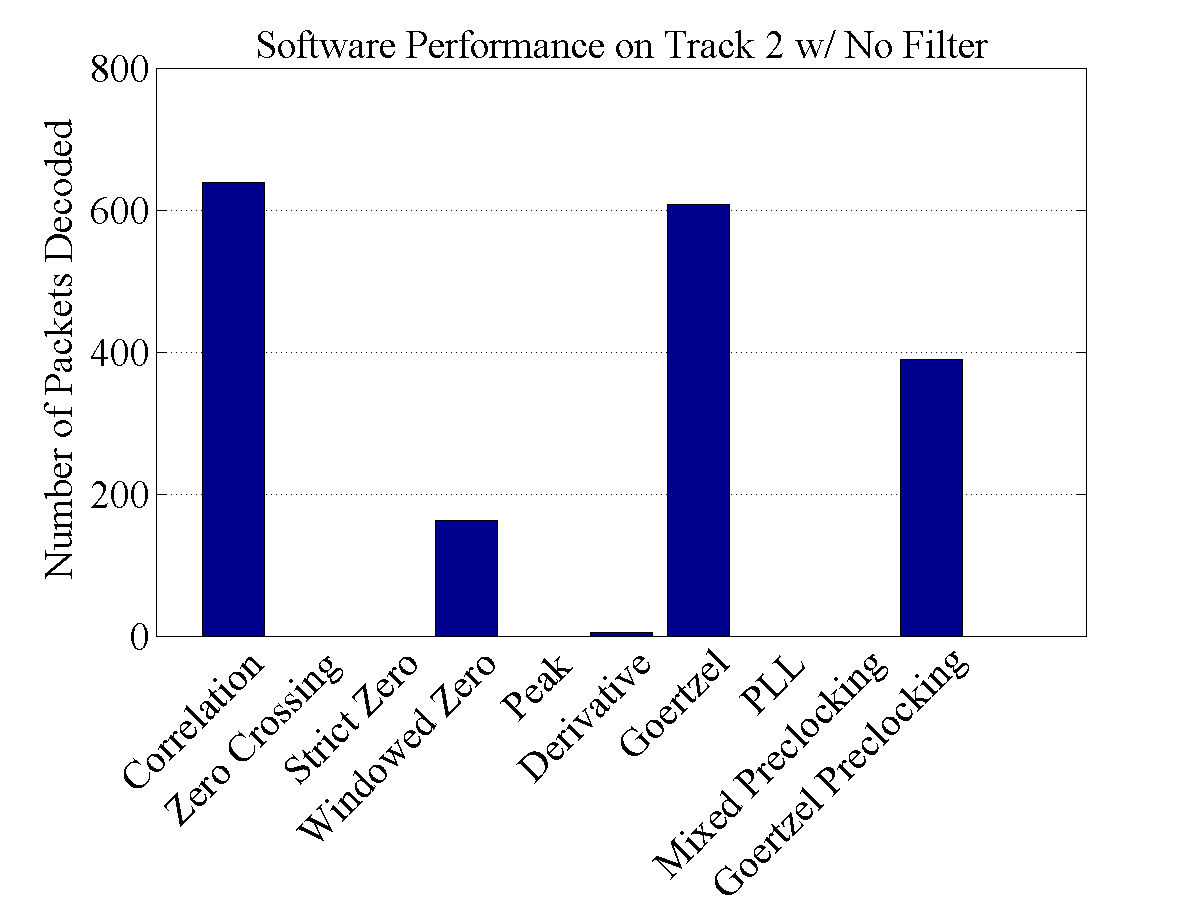
\includegraphics[width=0.75\linewidth]{images/SoftwarePerformanceonTrack2wNoFilter.png} 
	\caption{Performance of software on the raw signal from Track 2.}
   \label{T2FiltNo}
\end{figure}
\begin{figure}
  \centering
	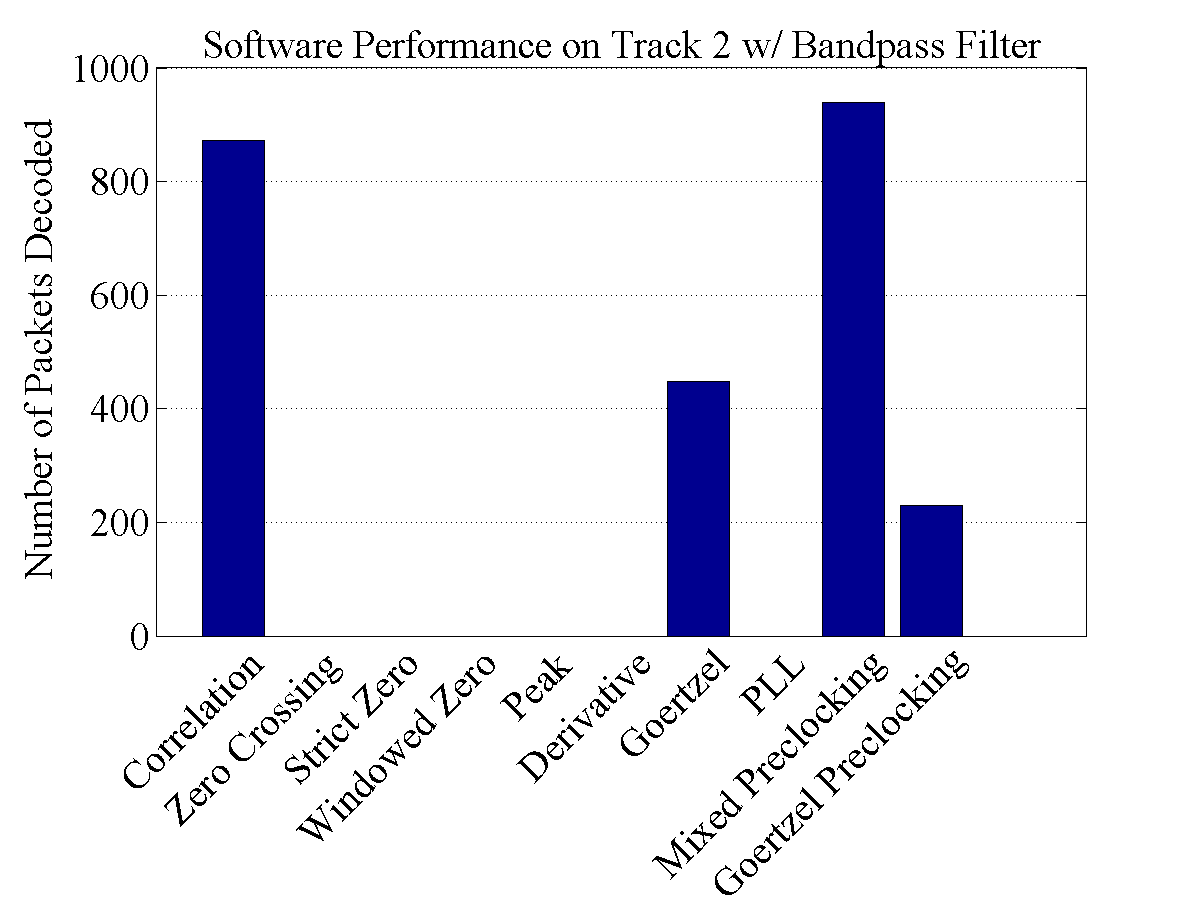
\includegraphics[width=0.75\linewidth]{images/SoftwarePerformanceonTrack2wBandpassFilter.png} 
	\caption{Performance of software on Track 2 with a bandpass filter.}
   \label{T2Filt0}
\end{figure}
\begin{figure}
  \centering
	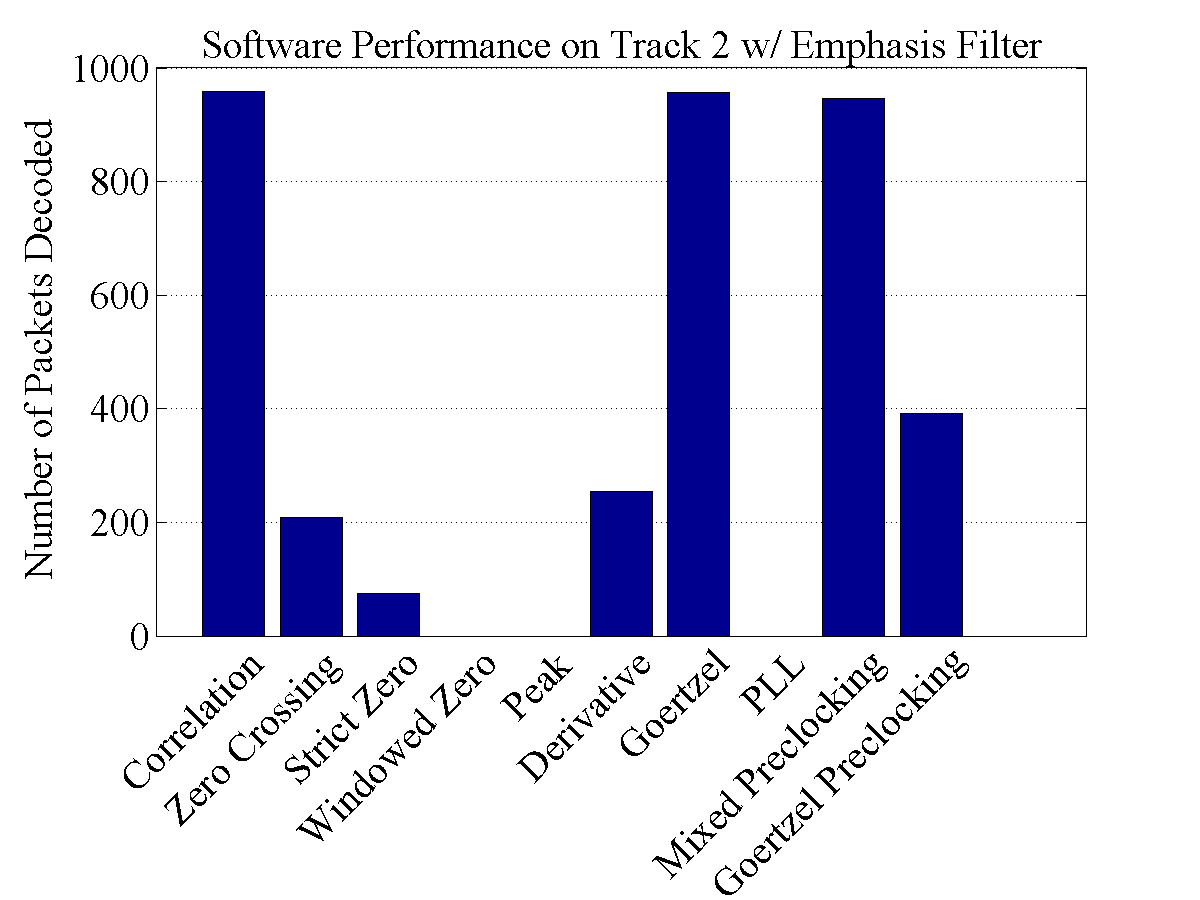
\includegraphics[width=0.75\linewidth]{images/SoftwarePerformanceonTrack2wEmphasisFilter.png} 
	\caption{Performance of software on Track 2 with an emphasis filter.}
   \label{T2Filt6}
\end{figure}


\subsection{Hardware and Software Comparisons}
It is now time to actually compare the new software implementations to the old ones as well as to the hardware. The first thing to notice is that the Goertzel Filter did very well, and in some cases better than the original correlation. Secondly, the complicated preclocking algorithm was also able to hold its own and still be a top contender. In fact the top three software algorithms were Correlation, Goertzel, and Mixed Preclocking with 964, 965, and 939 packets decoded from Track 1 with the bandpass filter. Even though they all have different number of packets decoded they each still have their expertise with being able to exclusively decode packets that others could not. For instance when the three are run together there is a total of 975 packets decoded due to the fact that Goertzel gets 12 packets that the other two do not, Correlation gets 7 that the others do not, and Preclocking decoded 3 that these other two missed. This could still be a good argument for the use of hardware over software since it is very easy to run multiple demodulators in parallel. Especially since the cost of this is only 5 minutes and 2 seconds on a file that is 25:49 long.

The question is, is the software better than the hardware? Looking at the highest numbers, no, but looking at the bigger picture, maybe. One thing about the hardware is that it is prone to variations and in need of periodic tuning. So, if instead of looking at the best of the breed, the average values are compared under the presumption that this would correspond to the average ham's decoding capabilities, then the software does decode more packets. Additionally, the software does not have any capacitors that will dry up or solder joints that may become brittle and affect the performance. The performance of the software today will be exactly the same in 5, 10, many years. The average number of packets decoded by the hardware on Track 1 was 935. Looking at this value any one of the three algorithms that are the top performers would be considered better.
